%=========================================================================
% (c) Michal Bidlo, Bohuslav Křena, 2008

%=========================================================================%
% - - - KAPITOLA 1: Ú V O D                                               %
\chapter{Úvod}                                                            %
%=========================================================================%
V dnešní době se na testování klade velký důraz, a proto je potřeba se touto částí vývoje software zabývat detailně. Aplikace lze testovat různými způsoby, od jednoduchých manuálních testů po sofistikované nástroje automaticky spouštějící vybrané sady testů. Pro tyto účely existuje mnoho nástrojů\footnote{\url{https://en.wikipedia.org/wiki/List_of_unit_testing_frameworks}}, které usnadňují programátorům práci. Cílem těchto nástrojů je redukce množství napsaného kódu opakujícího se v testech pro podobné komponenty nebo jejich vlastnosti.

Co se týče programovacího jazyka Java, můžeme vybírat z velkého množství nástrojů\footnote{\url{https://en.wikipedia.org/wiki/List_of_unit_testing_frameworks\#Java}} pro testování podle toho, jaký aspekt software chceme testovat. Pro testování Servler, Bean a Java tříd lze testovat pomocí nástrojů jako jsou například Servlets, JUnit, Arquillian, ServletUnit nebo Mock objects. Pro testování grafického uživatelského rozhraní vytvořeného pomocí Swing lze použít například UISpec4j, Abbot, Fest, QF-Test a další. Pro funkcionální testování lze použít například HTTPUnit, JWebUnit, TestNG a Selenium Webdriver, zatímco pro výkonnostní testování lze použít například Apache JMeter.

Tato práce se zabývá popisem infrastruktury vývojového prostředí Eclipse (dále zkráceně Eclipse IDE) a jeho zásuvných modulů s přihlédnutím k budoucímu použití pro vytvoření vlastního zásuvného modulu. Dále se zabývá popisem testovacího rámce JUnit a jeho architekturou. JUnit je snadno rozšiřitelný a je obsažen ve velkém množství testovacích nástrojů a vývojových prostředí včetně Eclipse IDE, kde ho lze použít při testování jeho grafického uživatelského rozhraní (dále zkráceně GUI). Klíčovou částí práce je návrh a implementace zásuvného modulu Eclipse IDE, který zpracovává data z testovacího rámce JUnit a posílá informace o průběhu testů do klientské aplikace, kde je zobrazuje uživateli. Důvodem pro tvorbu tohoto zásuvného modulu je potřeba programátora zjistit v jaké fázi se probíhající sada testů nachází, který test v dané chvíli běží a jak dopadly již proběhlé testy.


%=========================================================================%
% - - - KAPITOLA 2: V Ý V O J O V É - P R O S T Ř E D Í - E C L I P S E   %
\chapter{Vývojové prostředí Eclipse}                                      %
%=========================================================================%
Eclipse IDE je integrované vývojové prostředí poskytující podporu pro mnoho programovacích jazyků, jako jsou například Java, C, C++, Javascript a PHP.  Je záložen na modulové architektuře, která umožňuje snadné rozšíření této platformy. Pro přidání nové funkcionality do vývojového prostředí stačí nainstalovat příslušný zásuvný modul (\textsc{angl. plugin}). Projekt Eclipse je udržován radou správců eclipse.org, která vznikla z iniciativy společností Borland, IBM, MERANT, QNX Software Systems, Rational Software, Red Hat, SuSE, TogetherSoft a Webgain. Cílem eclipse.org je tvorba univerzálního rozšiřitelného IDE, které poskytuje nástroje pro integraci různých platforem a zároveň potřebné nástroje pro jejich tvorbu a rozšíření. 
%TODO: cite: https://eclipse.org/org/#history
V následující kapitole je popsána struktura Eclipse IDE a částí, ze kterých se skládá. Dále je zde popsán systém zásuvných modulů Eclipse IDE a jejich částí.

  \section{Infrastruktura Eclipse}
  %===============================
  Eclipse IDE není monolitické vývojové prostředí, ale spíše komplexní soubor zásuvných modulů. V základě je rozdělen do několika podsystémů, které jsou koncipovány jako jeden nebo více zásuvných modulů. Minimální množina zásuvných modulů, která je potřeba pro vývoj klientské aplikace se nazývá Eclipse RCP (Rich Client Platform)\footnote{\url{https://wiki.eclipse.org/Rich_Client_Platform}}. V dnešní době se však Eclipse IDE často používá i pro vývoj serverových aplikací, tato infrastruktura se potom nazývá EAF (Eclipse Aplication Framework)\cite{Plugins}. Důležitou komponentou je jádro, které načítá jednotlivé zásuvné moduly. Toto jádro je implementováno na základě specifikace OSGi Service Platform, která definuje standard pro dynamické modulární systémy v Javě. Tento standard je definován mezinárodním konsorciem OSGi Alliance\footnote{\url{https://www.osgi.org/}}. Díky implementaci rámce OSGi Equinox\footnote{\url{http://www.eclipse.org/equinox/}} používá Eclipse IDE pro načítání jednotlivých zásuvných modulů návrhový vzor lazy-loading, který zajišťuje načítání jen nezbytných zásuvných modulů. 
  
  \todo{Najít způsob jak dát následující větu jako samostatný blok textu.}
  Zásuvné moduly se v základu dělí podle funkce do několika skupin:
  \begin{description}
    \item[Core] je skupina nízkoúrovňových zásuvných modulů zajišťujících základní funkce jako jsou zpracování rozšíření zásuvných modulů a zdrojových kódů.
    \item[SWT (Standard Widget Toolkit)] je knihovna nástrojů pro manipulaci s uživatelským rozhraním, která poskytuje API nezávislé na operačním systému.
    \item[JFace] je knihovna přidávající další funkcionalitu jako nástavbu k SWT.
    \item[GEF] je rámec poskytující prostředí pro vývoj grafických editorů.
    \item[Workbench] obsahuje zásuvné moduly poskytující funkcionalitu specifickou přímo pro Eclipse IDE, jako je manipulace s projekty nebo grafickými prvky (pohledy, perspektivami, atd.).
    \item[Team] je skupina zásuvných modulů poskytujících podporu pro správu verzí v Eclipse IDE.
    \item[Help] poskytuje dokumentaci k jednotlivým prvkům Eclipse IDE.
    \item[JDT (Java Development Tools)\footnote{\url{http://www.eclipse.org/jdt/}}] slouží pro vývoj Javových aplikací- přidává podporu pro vývoj Java aplikací a navíc do Eclipse IDE přidává perspektivy, pohledy, průvodce a další nástroje pro práci s Javou.
    \item[PDE (Plug-in Development Enviroment)\footnote{\url{http://www.eclipse.org/pde/}}] je skupina zásuvných modulů poskytujících různé nástroje (pohledy, editory, atd.) pro práci se zásuvnými moduly a jejich manifesty.
    \item[Mylyn] poskytuje uživatelské rozhraní pro správu a prezentaci informací definovaných uživatelem.
  \end{description}

  Na obrázku \ref{fig:eclipse_arch} jsou znázorněny základní komponenty platformy Eclipse. Workbench představuje obálku, která umožňuje uživateli orientaci ve vývojovém prostředí. Definuje body rozšíření "Extension points", kde je možno k zásuvnému modulu přidat další, rozšiřující modul. Díky těmto bodům lze přidávat například komponenty grafického rozhraní, jako jsou pohledy, editory a menu. Pracovní plocha Workspace definuje API pro vytváření a správu projektů, souborů a složek. Zde jsou projekty překládány a sestavovány. Workspace navíc obsahuje další informace k projektům, jako je například uživatelské nastavení. Help poskytuje body rozšíření sloužící pro zobrazení nápovědy nebo dokumentace. Modul Team definuje model pro vývoj aplikací v týmu, s podporou správy verzí aplikace a zdrojových kódů. Platform Runtime dynamicky vyhledává zásuvné moduly a spravuje informace o nich a jejich bodech rozšíření.

  \begin{figure}[h]
    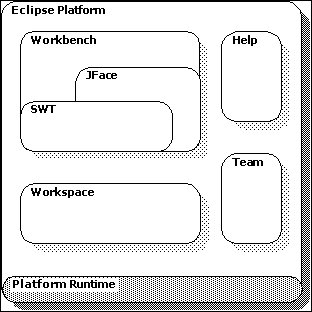
\includegraphics[width=0.5\textwidth, center]{obrazky-figures/eclipse_arch.jpg}
    \caption{Architektura platformy Eclipse.}
    \label{fig:eclipse_arch}
  \end{figure}

    \subsection{Workbench}
    %*********************
    Termín Workbench odkazuje na desktopové vývojové prostředí. Jeho cílem je integrace různých nástrojů a poskytnutí základního schématu pro tvorbu, správu a navigaci ve zdrojích pracovní plochy Workspace. Běžně se ve Workbench nachází lišta s hlavním menu, nástrojová lišta a několik pohledů, případně editorů. Grafické prvky vývojového prostředí jsou však pro uživatele přizpůsobitelné.

    \begin{figure}[h]
      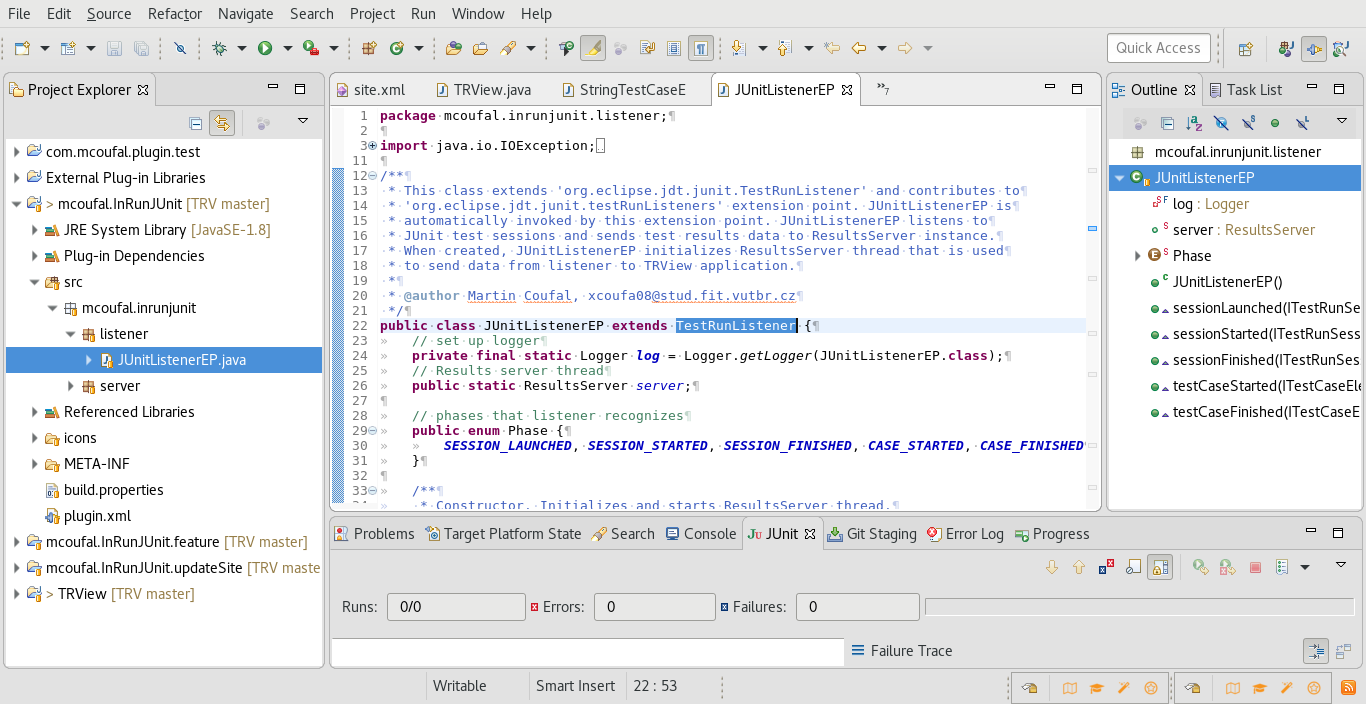
\includegraphics[width=0.7\textwidth, center]{obrazky-figures/eclipse_workbench.png}
      \caption{Běžný vzhled Eclipse Workbench.}
      \label{fig:eclipse_workbench}
    \end{figure}

    \subsection{Pohledy}
    %*******************
    Pohled je jednou ze základních komponent tvořících uživatelské rozhraní Eclipse. Slouží k zobrazování zdrojových souborů a informací uživateli a také k navigaci ve vývojovém prostředí. Každý pohled může mít svá menu a své nástrojové lišty.

      \subsubsection{Deklarace pohledu View}
      %-------------------------------------
      Pro vytvoření nového pohledu View je zapotřebí dvou kroků- vytvoření kategorie pohledu View (pokud ho nechceme vytvořit v některé z již existujících kategorií) a deklarace nového pohledu. Obě dvě změny probíhají v manifestu zásuvného modulu. Přesto, že je možné tyto změny do manifestu dopsat ručně, vývojové prostředí Eclipse nabízí praktické nástroje pro editaci manifestů zásuvných modulů. Otevření některého z manifestů zásuvného modulu spustí editor zásuvného modulu. Nastavení rozšíření zásuvného modulu lze upravovat v záložce \texttt{Extensions}. Pro přidání kategorie pohledu View  i deklarace pohledu View samotného je nutné nejdříve přidat správný bod rozšíření. Všechny pohledy View se připojují na bod rozšíření \texttt{org.eclipse.ui.views}. K tomuto bodu rozšíření lze přidat novou kategorii pohledu View, nebo deklarovat nový pohled View. Pro přidání kategorie je nutno zadat atributy \texttt{id} a \texttt{name}. Deklarace nového pohledu View vyžaduje atributy \texttt{category}, \texttt{class}, \texttt{icon}, \texttt{id} a \texttt{name}. 
      
      \subsubsection{Implementace třídy pohledu View}
      %----------------------------------------------
      Zdrojový kód s popisem chování daného pohledu View se nachází ve třídě implementující rozhraní \texttt{org.eclipse.ui.IViewPart}. Běžně používanou třídou implementující toto rozhraní je \texttt{org.eclipse.ui.part.ViewPart}. Pro zajištění správného chování nově vytvořeného pohledu je v této třídě zapotřebí definovat následující metody:
      \begin{itemize}
	\item \texttt{createPartControl(Composite)} \todo{Je vhodné popsat co která metoda dělá? Je ZDE správné místo? (Popřípadě lze použít definiční seznam)}
	\item \texttt{dispose()}
	\item \texttt{getAdapter(Class)}
	\item \texttt{saveState()IMemento}
	\item \texttt{setFocus()}
      \end{itemize}

      \todo{Zde mohou být další detaily k implementaci pohledu View (View controls, model, Content/Label provider, ...) - prozatím těžko říct zda budou relevantní k BP}
    
    \subsection{Perspektivy}
    %***********************
    Perspektivy slouží jako nástroj pro seskupení relevantních komponent v aktivním okně Workbench. Komponenty se seskupují podle úkonu, který bude uživatel vykonávat a  zároveň podle programovacího jazyka, ve kterém uživatel projekt vytváří. Pokud je to žádoucí, lze také při přidání nového zásuvného modulu některou z již existujících perspektiv pouze upravit.

    Pro přidání nové perspektivy, podobně jako u přidání nového pohledu View, je nutno do manifestu zásuvného modulu přidat správný bod rozšíření- \texttt{org.eclipse.ui.perspectives}. Rozložení komponent v dané perspektivě je definováno ve třídě implementující rozhraní \texttt{IPerspectiveFactory}. Přidat nové rozšíření zásuvného modulu implementující novou nebo upravenou perspektivu lze jednoduše pomocí nástrojů v záložce \texttt{Extensions} u editoru zásuvného modulu. Chceme-li perspektivu pouze upravit, lze při tvorbě nové perspektivy vybrat některou z již existujících.

    \subsection{Editory}
    %*******************
    Editory slouží jako hlavní nástroj pro úpravu zdrojového kódu a jiných textových souborů. Eclipse nabízí mnoho editorů, které je možno nainstalovat v rámci nějakého ze zásuvných modulů. Nejzákladnějším editorem je textový editor, který poskytuje pouze základní funkce pro práci s textem bez zvýraznění nebo kontroly syntaxe. I ten je však možno dále rozšířit pomocí dalších zásuvných modulů.

    Editor lze přidat pomocí rozšiřujícího bodu \texttt{org.eclipse.ui.editors}. Na ten lze připojit vlastní třídu implementující rozhraní \texttt{org.eclipse.ui.IEditorPart}. Proces vytváření nového editoru je stejný jako v předchozích dvou případech.

  \section{Architektura zásuvných modulů v Eclipse IDE}
  %====================================================
  Každý zásuvný modul v Eclipse IDE slouží buď jako knihovna pro dodatečné funkce jiným zásuvným modulům, nebo slouží pro rozšíření funkcionality platformy. Chování každého zásuvného modulu je popsáno v jeho zdrojovém kódu. Závislosti, body rozšíření a služby poskytované  zásuvným modulem jsou popsány v manifestech modulu- souborech \texttt{MANIFEST.MF} a \texttt{plugin.xml}. Načítání nových zásuvných modulů probíhá až když je modul přímo vyžadován (dle návrhového vzoru lazy-loading). V základu jsou načteny pouze manifesty, které poskytují základní informace o zásuvném modulu. Nemusí se tak načítat kompletní instalované zásuvné moduly a Eclipse IDE se tak spouští rychleji.

  Zásuvný modul (ať už v podobě Java archivu JAR nebo v podobě adresáře) se skládá z Javových tříd, manifestů zásuvného modulu (\texttt{MANIFEST.MF} a \texttt{plugin.xml}) a obrázkových souborů, typicky umístěných v adresářích pojmenovaných \texttt{icons} nebo \texttt{images}. Pokud je zásuvný modul ve formě adresáře, archiv JAR je uložen v některém z podadresářů. Název archivu JAR a jeho umístění je potom definováno v souboru \texttt{MANIFEST.MF}.

    \subsection{Model zásuvných modulů}
    %********************************
    Eclipse IDE při startu prohledá všechny adresáře se zásuvnými moduly a vytvoří vlastní model obsahující každý nalezený zásuvný modul. Tento model se vytváří pomocí manifestů zásuvných modulů tak, aby Elipse IDE nemusel načítat celé zásuvné modely a ušetřil tak čas a místo. Informace o jednotlivých nainstalovaných zásuvných modulech jsou uloženy v balíčcích (\textsc{angl. bundles}). Získáváním informací přes rozhraní těchto balíčků zajistíme, aby se zásuvné moduly nenačítaly, dokud nejsou opravdu zapotřebí.
    
    Původně mělo Eclipse IDE vlastní mechanismus pro běh aplikace, ale to znemožnilo použití již vytvořených technologií v jiných oblastech jako Avalon nebo JMX. Proto byl nakonec nahrazen mechanismem pro běh aplikace založeném na technologii OSGi Alliance, která poskytuje model s detailní specifikací a podporuje dynamické chování.\cite{Plugins}

    \subsection{Manifesty zásuvného modulu}
    %**************************************
    Manifesty zásuvného modulu jsou dva soubory- \texttt{MANIFEST.MF} a \texttt{plugin.xml}. První zmíněný obsahuje data nutná pro běh zásuvného modulu jako jsou identifikátor, verze a závislosti zásuvného modulu. Druhý obsahuje data ve formátu XML popisující případná rozšíření a body rozšíření. 

      \subsubsection{Manifest 'MANIFEST.MF'}
      %-------------------------------------
      V každém souboru \texttt{MANIFEST.MF} zásuvného modulu se nacházejí záznamy pro jméno, identifikátor, verzi, spouštěč a poskytovatele balíčku zásuvného modulu. Dále se zde mohou vyskytovat záznamy s cestou ClassPath, exportovanými balíčky a závislostmi zásuvného modulu.
      \todo{Nahradit slovní spojení cestou ClassPath něčím jiným - u ClassPath zde to není vhodný překlad.}
      Jméno (Bundle-Name) a poskytovatel (Bundle-Vendor) jsou "human-readable" řetězce, které nemusí být unikátní a lze je ukládat do zvláštního souboru \texttt{plugin.properties} za účelem internacionalizace.

      Identifikátor (Bundle-SymbolicName) slouží k jednoznačné identifikaci daného balíčku Bundle. Většinou se jako identifikátor balíčku Bundle používá Javová konvence pro pojmenování balíčků: "com.<název společnosti>.<komponenta>[.<část komponenty>]", kde část dané komponenty (například 'ui' nebo 'core') se uvádí v případě větších komponent, kde jsou jednotlivé balíčky rozděleny.
      
      Verze (Bundle-Version) slouží k jednoznačné identifikaci verze daného balíčku. V případě shody identifikátorů je vždy vybrán balíček s novějším číslem verze. Toto číslo se skládá ze 3 číslic oddělených tečkami a v případě potřeby i alfanumerického řetězce použitelného pro uzší specifikaci (například '1.2.3.beta'). První číslo označuje majoritní verzi produktu, druhé minoritní verzi produktu a třetí slouží k označení úrovně služeb.

      Spouštěč (Bundle-Activator) je volitelná část manifestu která umožňuje specifikovat třídu implementující rozhraní BundleActivator a poskytuje tak metody start() a stop(), které jsou přínosné pro správu životního cyklu balíčku Bundle.
      \todo{K plugin class by se dala napsat celá kapitola, ale asi to nebude relevantní vzhledem k BP}
      
      Cesta ClassPath (Bundle-ClassPath) je čárkami oddělený seznam knihoven ve formátu JAR obsahujících zdrojový kód zásuvného modulu.
      
      Záznam s exportovanými balíčky (Export-Package) je podmnožina knihoven z cesty ClassPath obsahující knihovny, které se mají exportovat, aby byly viditelné pro ostatní zásuvné moduly.
      
      Eclipse IDE vytváří pro každý načtený zásuvný modul novou instanci pro načtení třídy, která slouží k vyhledávání a načítání zásuvných modulů a používá záznam závislostí v manifestu k určení viditelnosti ostatních zásuvných modulů. Záznam závislostí (Require-Bundle) je seznam zásuvných modulů, které jsou pro daný zásuvný modul viditelné z hlediska vykovávání programu. 
      
      \subsubsection{Manifest 'plugin.xml'}
      %------------------------------------
      V tomto manifestu zásuvného modulu mohou být uvedeny body rozšíření, na které je možno připojit nový zásuvný modul rozšiřující stávající funkcionalitu. Toto odloučení od rozšiřujících zásuvných modulů umožňuje existenci základního zásuvného modulu bez znalosti jakýchkoliv informací o ostatních zásuvných modulech. To zajišťuje snazší spolupráci při implementaci a znovupoužitelnost již implementovaných částí. Rozšiřující bod obvykle definuje identifikátor, jméno a schéma. To určuje, co musí rozšiřující zásuvný modul splnit pro správné rozšíření tohoto zásuvného modulu.\todo{Možno přidat sample kódu jak vypadá rozšiřující bod.}
      
      Dále je zde možno definovat, který zásuvný modul chceme stávajícím modulem rozšířit. K tomu slouží rozšíření zásuvného modulu (viz obrázek ...\todo{Vytvořit screenshot kódu - popřípadě napsat sample kódu.}) 

%=========================================================================%
% - - - KAPITOLA 3: J U N I T                                             %
\chapter{JUnit}                                                           %
%=========================================================================%
\todo{Popsat více do detailu, přidat odkaz na nástroje rozšiřující JUnit.}
JUnit je jednoduchý nástroj pro psaní testů a testování aplikací. Jeho vývoj je založen na otevřeném zdrojovém kódu (open-source), a proto lze najít další nástroje, které rámec JUnit používají nebo z něj vycházejí. Cílem JUnit je poskytovat nástroj, který umožní:
\begin{description}
  \item[Jednoduchost psaní testů]
  Programátor nemusí psát zbytečně mnoho kódu, zbytek za něj vykoná rámec JUnit.
  \item[Snadné pochopení rámce JUnit]
  Lorem ipsum dolor sit amet.
  \item[Rychlé provedení testů]
  Lorem ipsum dolor sit amet.
  \item[Izolované provedení testů]
  Lorem ipsum dolor sit amet.
  \item[Skládat a provádět různé kombinace testů]
  Lorem ipsum dolor sit amet.
\end{description}

Bohužel jsou některé z těchto podmínek v rozporu mezi sebou a tak nelze splnit všechny z těchto požadavků naplno.
  
  \section{Architektura rámce JUnit}
  %=================================
  Lorem ipsum dolor sit amet.
  
    \subsection{xUnit}
    %*****************
    % Vychazi z xUnit - popsat navrh xUnit + jak vynikl SUnit (odkaz na praci K. Becka Simple Smalltalk Testing: With Patterns)
    Lorem ipsum dolor sit amet.
    
    \subsection{JUnit}
    %*****************
    % Popis architektury / implementace JUnit 
    Lorem ipsum dolor sit amet.
  
  \section{Rozšíření rámce JUnit}
  %==============================
  Lorem ipsum dolor sit amet.
  
  \section{Zásuvné moduly Eclipse IDE rozšiřující rámec JUnit}
  %===========================================================
  Lorem ipsum dolor sit amet.
  % Zminit jake moduly rozsiruji JUnit a jak, detailneji popsat jen ten co pouziji.
    \subsection{Zásuvný modul org.junit.???}
    %***************************************
    Lorem ipsum dolor sit amet.
    \subsubsection{JUnit ui}
    %-----------------------
    % Tady by mela byt popsana zakladni struktura daneho pluginu + Tridy dulezite z hlediska implementace 
    Lorem ipsum dolor sit amet.
    \subsubsection{JUnit core}
    %-------------------------
    % Tady by mela byt popsana zakladni struktura daneho pluginu + Tridy dulezite z hlediska implementace
    Lorem ipsum dolor sit amet.
    
%=========================================================================%
% - - KAPITOLA 4: Z Á S U V N Ý - M O D U L - I n R u n J U n i t V i e w %
\chapter{Implementovaný zásuvný modul}                                    %
%=========================================================================%
Díky architektuře zásuvných modulů je snadné rozšířit Eclipse IDE o novou funkcionalitu, tu je ale potřeba otestovat. V rámci testováni grafického uživatelského rozhraní Eclipse IDE se používají rozsáhlé testovací sady testující velké množství aspektů a možností. Automatické testy grafického uživatelského rozhraní jsou časově náročné a nejsou dokonalé. Vzniká tak potřeba kontroly nad sadou s probíhajícími testy. Pokud jsou testy spouštěny z grafického uživatelského rozhraní Eclipse IDE, lze průběh testů sledovat pomocí zásuvného modulu \todo{Doplnit název} ,který poskytuje pohled JUnit zobrazující potřebné informace o probíhajících testech. Nejen z hlediska časové náročnosti však může být výhodnější testovat na vzdálených serverech a spouštět testy z terminálu. V takovém případě nelze použít pohled JUnit k zobrazení detailů o testování.

Jedním z častých problémů při testování grafického uživatelského rozhraní je nedokonalost izolace jednotlivých testů v testovací sadě. Může se tak stát, že některý z testů zanechá testovanou instanci v nekorektním stavu a následující testy selžou. Dalším problémem může být zacyklení některého z testů v testovací sadě. \todo{ DOPSAT!}
Důležitými faktory, které by měla tato kontrola obsahovat, jsou zejména zobrazení průběhu a výsledků testů v rámci spuštěné testovací sady. To zajistí\todo{carka?Zmenit to zajisti-zni to divne} aby v případě nějaké chyby v testovací sadě měl programátor možnost lépe prozkoumat kde chyba nastala a napravit ji.

Implementovaný zásuvný modul InRunJUnitView poskytuje možnost zobrazení stejnojmeného pohledu, který zobrazuje informace o probíhajícím testování přímo v testované instanci. Tato kapitola detailně popisuje architekturu, implementaci, způsob testování a využití tohoto zásuvného modulu.

\todo{Vytvořit diagram znázorňující funkci zásuvného modulu při testování na vzdáleném serveru.}
\begin{figure}[!h]
  
\includegraphics[width=\textwidth, center]{obrazky-figures/placeholder.pdf}
  \caption{Funkce zásuvného modulu InRunJUnitView.}
  \label{fig:inrunjunitview_principle}
\end{figure}
V následující kapitole je uvedena architektura, implementace a popis testování zásuvného modulu InRunJUnitView. Ten vytváří pohled View v testované instanci EclipseIDE, který zobrazuje průběh testovaní této instance.


  \section{Návrh architektury zásuvného modulu}
  %============================================
  \todo{Popis proč jsem vybral zrovna toto řešení.}
  
  Zásuvný modul se skládá ze dvou hlavních částí, \texttt{core} a \texttt{ui}. První část slouží k získání výsledků o průběhu testu, jejich zpracování a odeslání do testované instance Eclipse IDE. Výsledek se získává z rámce JUnit pomocí instance třídy \texttt{TestListener}. Z této instance lze získat výsledek typu \texttt{Result}. Ten je poslán druhé části zásuvného modulu. Druhá část zásuvného modulu čeká na výsledky zaslané z \texttt{core}, které následně zpracovává a zobrazuje v běžící instanci Eclipse IDE do pohledu InRunJUnitView. Pro správnou funkci tohoto zásuvného modulu je nutné z testované instance otevřít pohled InRunJUnitView a zajistit, aby byl viditelný a nekolidoval s testovanými prvky. Toto lze zajistit pomocí testovacího rámce nebo přímo z prováděného testu.

  \todo{Vytvořit diagram který znázorňuje architekturu zásuvného modulu}.
  \begin{figure}[!h]
    
\includegraphics[width=\textwidth, center]{obrazky-figures/placeholder.pdf}
    \caption{Znázornění architektury zásuvného modulu InRunJUnitView.}
    \label{fig:inrunjunitview_principle}
  \end{figure}

  
  \section{Implementace}
  %=====================
  Lorem ipsum dolor sit amet.
  \section{Testování}
  %==================
  Lorem ipsum dolor sit amet.

  \section{Praktické využití}
  %=========================
  Lorem ipsum dolor sit amet.

    \subsection{Použití při testování Eclipse v~RedHat}
    %**************************************************
    Lorem ipsum dolor sit amet.

    \subsection{Jiná využití}
    %************************
    Lorem ipsum dolor sit amet.

  \section{Možná rozšíření}
  %========================
  Lorem ipsum dolor sit amet.

%=========================================================================%
% - - - KAPITOLA 5: Z Á V Ě R                                             %
\chapter{Závěr}                                                           %
%=========================================================================%
Závěrečná kapitola obsahuje zhodnocení dosažených výsledků se zvlášť vyznačeným vlastním přínosem studenta. Povinně se zde objeví i zhodnocení z~pohledu daalšího vývoje projektu, student uvede náměty vycházející ze zkušeností s~řešeným projektem a uvede rovněž návaznosti na právě dokončené projekty.

%=========================================================================
